\documentclass[10pt,a4paper]{article}
\usepackage[latin1]{inputenc}
\usepackage{amsmath}
\usepackage{amsfonts}
\usepackage{amssymb}
\usepackage{pgf}
\usepackage{hyperref}
\usepackage{listings}
\usepackage{xfrac}
\let\underscore\_
\newcommand{\myunderscore}{\renewcommand{\_}{\underscore\hspace{0pt}}}
\myunderscore
\lstset{language=Python, numbers=left, numberstyle=\tiny\color{gray}, numbersep=3pt, escapeinside={\$}, basicstyle=\footnotesize\ttfamily, escapeinside={\%*}{*)}, breaklines=true}

\definecolor{darkgreen}{rgb}{0,0.7,0}

\newif\ifdraft
\drafttrue
%\draftfalse                                                                              
\ifdraft
\newcommand{\katznote}[1]{ {\textcolor{blue}    { ***Dan:      #1 }}}
\newcommand{\zhaonote}[1]{{\textcolor{darkgreen}    { ***Zhao:      #1 }}}
\newcommand{\note}[1]{ {\textcolor{red}    {\bf #1 }}}
\else
\newcommand{\katznote}[1]{}
\newcommand{\zhaonote}[1]{}
\newcommand{\note}[1]{}
\fi


\title{Application Skeleton Tool, v 1.1}
\author{Zhao Zhang, Daniel S. Katz \\
University of Chicago \\
\{zhaozhang@uchicago.edu, dsk@uchicago.edu\}}

\begin{document}

\maketitle


This document introduces the Application Skeleton tool, part of the AIMES project. The report includes an introduction of the tool, examples of how it can be used, a user manual, and some future activities.

\newpage

\tableofcontents

\newpage

\section{Introduction}

The Application Skeleton (just `Skeleton' hereafter) tool \cite{Skeleton2013, Skeleton2014} lets users quickly and easily produce a synthetic distributed application that runs in a distributed environment, e.g. grids, clusters, clouds. The source code can be accessed at \url{https://github.com/applicationskeleton/Skeleton}.
A skeleton application is a synthetic application that is intended to represent the computation, I/O, and networking behavior of a real application.
In the Skeleton tool, an application is composed of one or more stages.
The user needs to define each stage's task type, number of processes, task length, computation and I/O interleaving option, read/write buffer size, input source, input size, output size, and other properties.

The Skeleton tool reads an application description file as input, and produces three groups of outputs: 
\begin{itemize}

\item[] \textbf{Preparation Scripts}: The preparation scripts are run to produce the input/output directories and input files for the synthetic applications.

\item[] \textbf{Executables}: Executables are the tasks of each application stage. (We assume different stages use different executables.)

\item[] \textbf{Application}: The overall application can be expressed in three different formats: shell commands, a Pegasus DAG, and a Swift script.
The shell commands can be executed in sequential order on a single machine.
The Pegasus DAG and the Swift script can be executed on a local machine or in a distributed environment.
Executing the Pegasus DAG or Swift script requires Pegasus or Swift, respectively.

\end{itemize}

\section{Examples}

Four examples of how the Skeleton tool can be used to build application skeletons follow, for a bag-of-tasks application, a multi-stage application, a MapReduce application, and an iterative application.  


\subsection{Bag-of-tasks application}

Listing~\ref{lst:bag} shows a sample input for a bag-of-tasks application with uniform task length, and uniform input and output file size, where each task reads one file and writes one file. Figure~\ref{fig:bag} shows the very simple DAG for this. The sample application description file can be accessed at \url{https://github.com/applicationskeleton/Skeleton/blob/master/src/sample-input/bag.input}.

\begin{lstlisting}[caption=Sample input for a bag-of-tasks application, label=lst:bag, linewidth=1.0\textwidth, xleftmargin=2.5ex]
Num_Stage = 1

Stage_Name = Bag
    Task_Type = serial
    Num_Tasks = 4  
    Num_Processes = 1
    Task_Length = uniform 5
    Read_Buffer = 65536
    Write_Buffer = 65536
    Input_Source = filesystem
    Input_Files_Each_Task = 1
    Tasks_Each_Input_File = 1
    	Input_1.Source = filesystem
    	Input_1.Size = uniform 1048576
    Output_Files_Each_Task = 1
        Output_1.Size = uniform 1048576
    Interleave_Option = 0    

\end{lstlisting}

\begin{figure}
   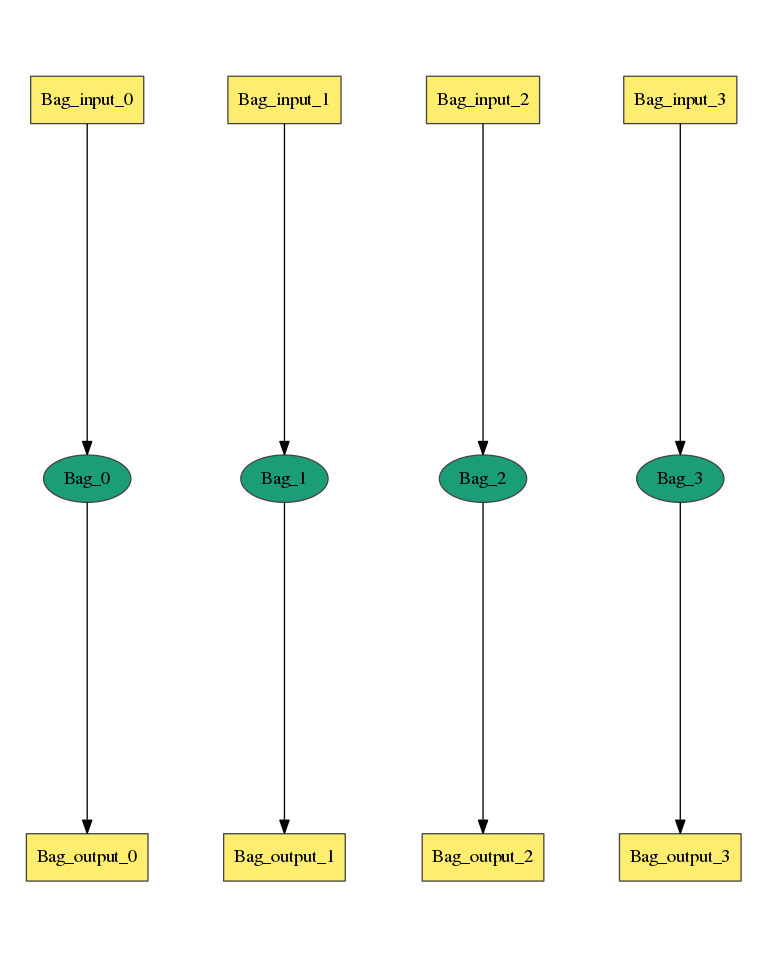
\includegraphics[width=120mm]{picture/bag}
\caption {Task flow of an bag-of-task application 
   \label{fig:bag}
}
\end{figure}


\subsection{Multi-stage application}

Listing~\ref{lst:sample} shows a three-stage application description file. The first stage has four tasks. Each reads two distinct files as input, runs for some time, and produces an output
file. The runtime for each task has a normal distribution, described by a two-value tuple: [average, stdev]. The input and output file size have a similar distribution. (Supported distributions
currently include: uniform, normal, gauss, triangular, lognorm, as further discussed in \S\ref{sec:distr}.) The second stage has six tasks. For each, the input file is the output of the first stage, as defined in Line 16, and the mapping between input 
files and tasks in the second stage is an all-pairs combination. (Mapping is discussed further in \S\ref{sec:def_mapping}.) The mapping is determined by the parameter \textbf{Input\_Task\_Mapping}. 
The third stage has only one task. 
It reads the six input files that were the output files from the second stage, and produces a single output file.


\begin{lstlisting}[caption=Sample input for a three-stage application, label=lst:sample, linewidth=1.0\textwidth, xleftmargin=2.5ex]
Num_Stage = 3

Stage_Name = Stage_1
    Task_Type = serial
    Num_Tasks = 4  
    Task_Length = normal [10, 1]
    Num_Processes = 1
    Read_Buffer = 65536
    Write_Buffer = 65536
    Input_Files_Each_Task = 2
        Input_1.Source = filesystem
        Input_1.Size = normal [10485760, 1048576]
        Input_2.Source = filesystem
        Input_2.Size = normal [10485760, 1048576]
    Output_Files_Each_Task = 1
        Output_1.Size = uniform 1048576
    Interleave_Option = 0

Stage_Name = Stage_2
    Task_Type = serial
    Num_Tasks = 6
    Task_Length = uniform 32
    Num_Processes = 1
    Read_Buffer = 65536
    Write_Buffer = 65536
    Input_Files_Each_Task = 2
    Input_Task_Mapping = combination Stage_1.Output_1 2
    Output_Files_Each_Task = 1
        Output_1.Size = uniform 1048576
    Interleave_Option = 0

Stage_Name = Stage_3
    Task_Type = serial
    Num_Tasks = 1
    Task_Length = uniform 32
    Num_Processes = 1
    Read_Buffer = 65536
    Write_Buffer = 65536
    Input_Files_Each_Task = 6
    Input_Task_Mapping = combination Stage_2.Output_1 6
    Output_Files_Each_Task = 1
        Output_1.Size = uniform 1048576
    Interleave_Option = 0    
\end{lstlisting}


Figure~\ref{fig:sample} shows the task flow of the synthetic application that is produced by the Skeleton tool with Listing~\ref{lst:sample} as input file.

\begin{figure}
   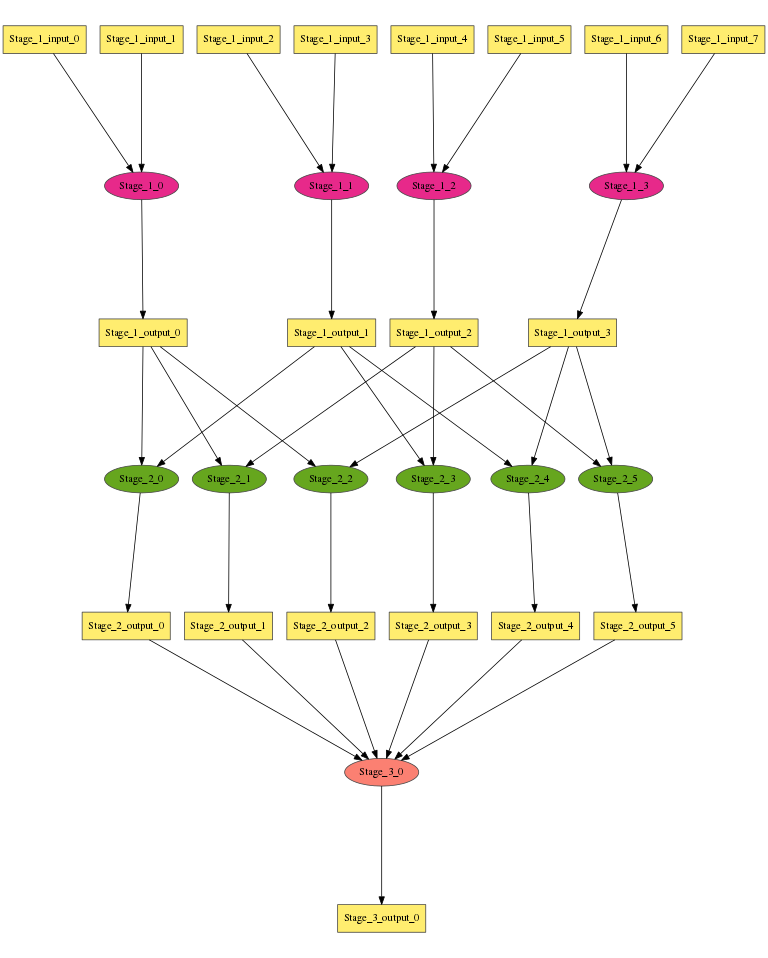
\includegraphics[width=120mm]{picture/sample}
\caption {Task flow of the three-stage application
   \label{fig:sample}
}
\end{figure}


\subsection{MapReduce application}
Listing~\ref{lst:mr} shows an input file for a MapReduce application.
Each map task reads one file and writes one file. 
Each Shuffle task task runs a fixed amount of time, representing reorganizing the file contents based on the hash value of some key in the file (the key can be a column in the text file). 
Each of these tasks reads all of the output files of the map tasks, and writes one output file (representing the records with hash values that fall in the task's range).
The two Reduce tasks read the outputs of all shuffle tasks, run a fixed amount of time, and write two distinct output files of fixed size. The Gather stage has one task that reads the output files from stage 3 and writes one output file (representing a combination of its inputs).
Figure~\ref{fig:mr} shows the DAG for this skeleton.
The sample application description file can be accessed at \url{https://github.com/applicationskeleton/Skeleton/blob/master/src/sample-input/map-reduce.input}.

\begin{lstlisting}[caption=Sample input for a MapReduce application, label=lst:mr, linewidth=1.0\textwidth, xleftmargin=2.5ex]
Num_Stage = 4

Stage_Name = Stage_1
    Task_Type = serial
    Num_Tasks = 4
    Task_Length = uniform 10
    Num_Processes = 1
    Read_Buffer = 65536
    Write_Buffer = 65536
    Input_Files_Each_Task = 1
        Input_1.Source = filesystem
        Input_1.Size = uniform 1048576
    Output_Files_Each_Task = 1
        Output_1.Size = uniform 1048576
    Interleave_Option = 0

Stage_Name = Stage_2
    Task_Type = serial
    Num_Tasks = 4
    Task_Length = uniform 32
    Num_Processes = 1
    Read_Buffer = 65536
    Write_Buffer = 65536
    Input_Files_Each_Task = 1
    Input_Task_Mapping = combination Stage_1.Output_1 4
    Output_Files_Each_Task = 1
        Output_1.Size = uniform 1048576
    Interleave_Option = 0

Stage_Name = Stage_3
    Task_Type = serial
    Num_Tasks = 2
    Task_Length = uniform 32
    Num_Processes = 1
    Read_Buffer = 65536
    Write_Buffer = 65536
    Input_Files_Each_Task = 2
        Input_1.Source = Stage_2.Output_1
	Input_2.Source = Stage_2.Output_1
    Output_Files_Each_Task = 1
        Output_1.Size = uniform 1048576
    Interleave_Option = 0

Stage_Name = Stage_4
    Task_Type = serial
    Num_Tasks = 1
    Task_Length = uniform 32
    Num_Processes = 1
    Read_Buffer = 65536
    Write_Buffer = 65536
    Input_Files_Each_Task = 2
        Input_1.Source = Stage_3.Output_1
	Input_2.Source = Stage_3.Output_1
    Output_Files_Each_Task = 1
        Output_1.Size = uniform 1048576
    Interleave_Option = 0

\end{lstlisting}

\begin{figure}
   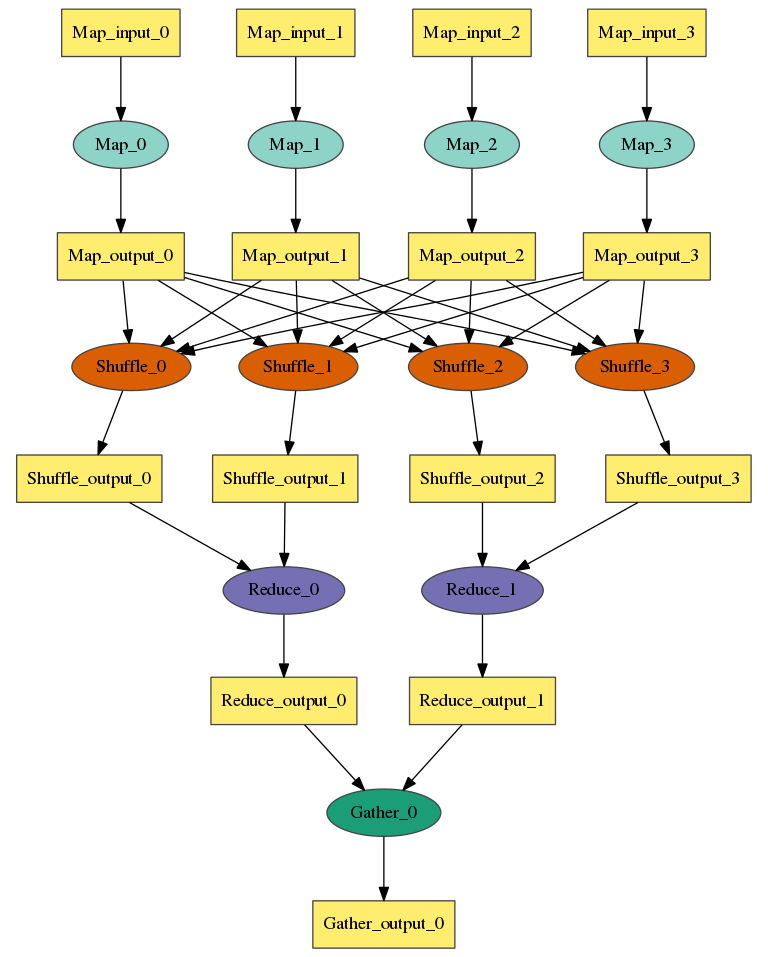
\includegraphics[width=120mm]{picture/mr}
\caption {Task flow of an MapReduce application with Stage\_1 referred as Map, Stage\_2 referred as Shuffle, Stage\_3 referred as Reduce, and Stage\_4 referred as Gather
   \label{fig:mr}
}
\end{figure}


\subsection{Iterative application}

The Skeleton tool can generate single-stage and multi-stage iterative applications, in both cases with a fixed number of iterations currently. To enable the iterative option,
users need to specify three additional parameters: \textbf{Iteration\_Num}, \textbf{Iteration\_Stages}, and \textbf{Iteration\_Substitute}. 
\textbf{Iteration\_Num} specifies 
the number of iterations of the target stage.\textbf{Iteration\_Stages} specifies the target stage(s). \textbf{Iteration\_Substitute} specifies the substitution
of input files of the target stage with the output files of latter stages.

Listing~\ref{lst:single-iter} shows a single-stage iteration example, in this case where the state is iterated three times, using the output from the previous iteration as the input for the second and third iterations. Figure~\ref{fig:single-iter} shows the visualized data flow.

\begin{lstlisting}[caption=Sample input for a single stage iterative application, label=lst:single-iter, linewidth=1.0\textwidth, xleftmargin=2.5ex]
Num_Stage = 1

Stage_Name = Stage_1
    Task_Type = serial
    Num_Tasks = 4
    Task_Length = uniform 10
    Num_Processes = 1
    Read_Buffer = 65536
    Write_Buffer = 65536
    Input_Files_Each_Task = 1
        Input_1.Source = filesystem
        Input_1.Size = uniform 1048576
    Output_Files_Each_Task = 1
        Output_1.Size = uniform 1048576
    Interleave_Option = 0
    Iteration_Num = 3
    Iteration_Stages = Stage_1
    Iteration_Substitute = Stage_1.Input_1, Stage_1.Output_1
 
\end{lstlisting}

\begin{figure}
   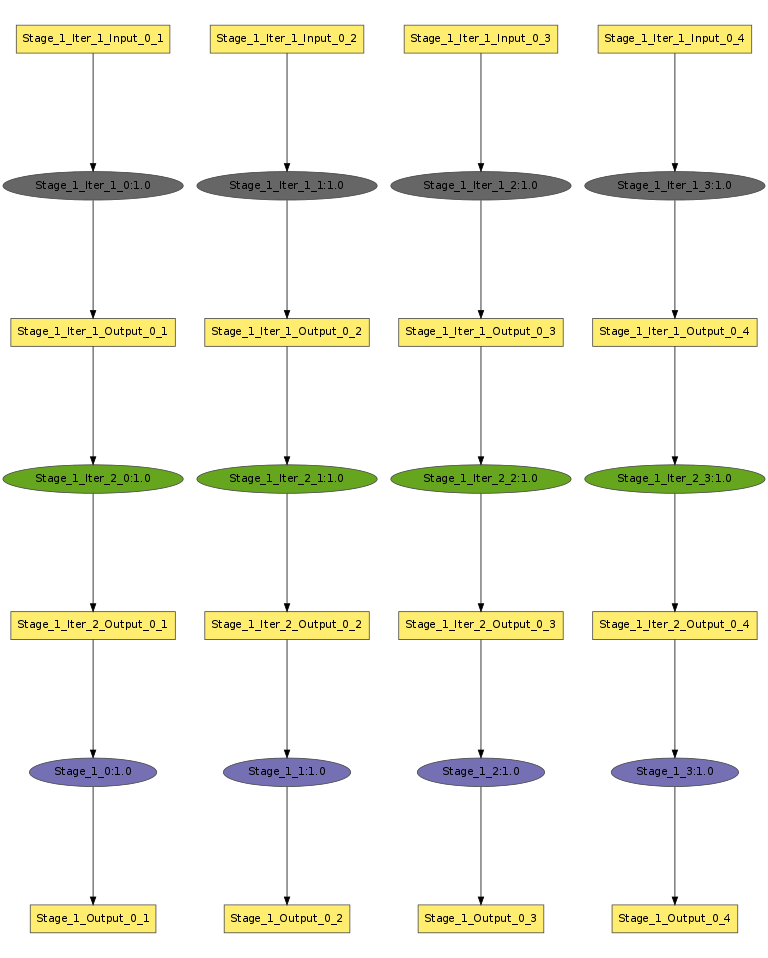
\includegraphics[width=120mm]{picture/single-iterate}
\caption {Task flow of a single stage iterative application
   \label{fig:single-iter}
}
\end{figure}



\section{User manual}

This section documents how a user can run the Skeleton tool and the available parameters to describe an application or an application stage.

\subsection{Requirements}

The Skeleton code is built to use Python3.  To use Python2 instead, please follow the instructions in the skeleton source file (\url{https://github.com/applicationskeleton/Skeleton/blob/master/src/skeleton.py}). 

\subsection{Application-wide parameter}

There is only one parameter that spans the whole description file:

\begin{itemize}

\item{\textbf{Num\_Stage}:} defines the total number of stages on this application.

\end{itemize}

\subsection{Stage-wide parameters}\label{sec:stage-wide}

Parameters documented in this section is only valid within its stage declaration scope.

\begin{itemize}

\item{\textbf{Stage\_Name}:} declares the stage name, e.g. Stage\_1.

\item{\textbf{Task\_Type}:} declares the task type (serial or parallel).

\item{\textbf{Num\_Processes}:} declares the number of processes in each task. If \textbf{Task\_Type} is serial, then \textbf{Num\_Processes} has to be ``1''. If \textbf{Task\_Type} is parallel, then \textbf{Num\_Processes} can be an integer value that is greater or equal to 1.

\item{\textbf{Num\_Tasks}:} declares the number of tasks in the stage.

\item{\textbf{Task\_Length}:} declares the length of the tasks in the stage. The distribution of task lengths can be uniform, normal, gauss, triangular, or lognorm. The distribution of task lengths can be a function of the input file size if and only if there is one input file per task. Please refer to \S\ref{sec:distr} for details.

\item{\textbf{Read\_Buffer}:} specifies the read buffer of each task, with default unit of bytes. e.g., 65536.

\item{\textbf{Write\_Buffer}:} specifies the write buffer of each task, with default unit of bytes. e.g., 65536.

\item{\textbf{Input\_Files\_Each\_Task}:} declares the ratio between number of input files and the number of tasks.


\item{\textbf{Input\_\$.Source}:} declares the input source of the \$th (i.e., 1 = first, 2 = second, 3=third, etc.) input file, either filesystem, or outputs of a previously defined stage (e.g., {\tt Input\_\$1.Source = Stage\_1.Output\_1}). 

\item{\textbf{Input\_\$.Size}:}  declares input file size of the  \$th input file. The distribution of task lengths can be uniform, normal, gauss, triangular, or lognorm. This parameter has to appear in pairs with \textbf{Input\_\$.Source}. (e.g., {\tt Input\_\$1.Size = uniform 1048576})

\item{\textbf{Input\_Task\_Mapping}:} declares user specified input file and task mapping. The mapping option currently only supports combination mapping and external mapping. 
Combination mapping lets users specify the input files in combinations and map to tasks. Please refer to Line 27 in Listing~\ref{lst:sample} for an example.
External mapping requires an executable that writes file grouping to standard output, with each group of file in a single line, delimited by spaces. Please refer to \S\ref{sec:def_mapping} for details and examples.

\item{\textbf{Output\_Files\_Each\_Task}:} declares the number of output files per task in the stage. (Multiple tasks writing to one file are not currently supported.)

\item{\textbf{Output\_\$.Size}:}  declares output file size for the stage. The distribution of task lengths can be uniform, normal, gauss, triangular, or lognorm. 

\item{\textbf{Interleave\_Option}:} the interleaving option of the task.
Please refer to \S\ref{sec:inter} for details.

\item{\textbf{Iteration\_Num}:} optional parameter specifying the number of iterations of one or more stages.

\item{\textbf{Iteration\_Stages}:} the names of the stages involved in the iteration, including the current stage. 

\item{\textbf{Iteration\_Substitute}:} the source and target files for substitution in iterations. (e.g., Line 18 in Listing~\ref{lst:single-iter}). 

\end{itemize}

\subsubsection{Distributions}\label{sec:distr}

The skeleton tool implements two types of distributions.

The first type, statistical distributions, can be used for \textbf{Task\_Length}, \textbf{Input\_\$.Size}, and \textbf{Output\_\$.Size}.

The second type, dependent distributions, can be used for \textbf{Task\_Length} and \textbf{Output\_\$.Size}.  \textbf{Task\_Length} can be a function of \textbf{Input\_\$.Size}, and \textbf{Output\_\$.Size} can be a function of  \textbf{Task\_Length} or \textbf{Input\_\$.Size}.

\paragraph{Statistical distributions}

If \textbf{Task\_Length}, \textbf{Input\_\$.Size}, and \textbf\textbf{Output\_\$.Size} are to be described as statistical distributions, one of the following distributions and formats should be used:

\begin{itemize}

\item{\textbf{uniform}}: [number], e.g. 5

\item{\textbf{normal}}: [avg, stdev], e.g. [5, 1]

\item{\textbf{gauss}}: [avg, stdev], e.g. [5, 1]

\item{\textbf{triangular}}: [avg, stdev], e.g. [5, 1]

\item{\textbf{lognorm}}: [avg, stdev], e.g. [5, 1]

\end{itemize}
For details, users may refer to \url{http://docs.python.org/3.3/library/random.html}

\paragraph{Dependent distributions}
\subparagraph{Task length as a function of input file size:} 

The \textbf{Task\_Length} can be a function of \textbf{Input\_\$.Size} if and only if there is one input file per task. The format to describe this option is:
\begin{itemize}
\item{\textbf{input}}: [coefficient, power], e.g. [4, 2]
\end{itemize}
where task length is computed as: \( \text{coefficient} * \text{filesize} ^ \text{power}\). 
Listing~\ref{lst:inputfunc} shows a sample code for this.

\begin{lstlisting}[caption=Use case of task length as a function of input file size, label=lst:inputfunc, linewidth=1.0\textwidth, xleftmargin=2.5ex]
Num_Stage = 1

Stage_Name = Stage_1
    Task_Type = serial
    Num_Tasks = 4  
    %*\texttt{\textbf{Task\_Length = polynomial [4, 2] Input\_1}}*)
    Num_Processes = 1
    Read_Buffer = 65536
    Write_Buffer = 65536
    Input_Files_Each_Task = 1
        Input_1.Source = filesystem
        Input_1.Size = uniform 5
    Output_Files_Each_Task = 1
    Output_File_Size = uniform 1048576
\end{lstlisting}

\subparagraph{Output file size as a function of input file size or task length:}
The \textbf{Output\_File\_Size} can be a function of either \textbf{Input\_File\_Size} or \textbf{Task\_Length}. The formats to describe these two options are:
\begin{itemize}
\item{\textbf{input}}: [coefficient, power], e.g. [4, 2]
\item{\textbf{length}}: [coefficient, power], e.g. [4, 2]
\end{itemize}
where output file size is computed as either 
\( \text{coefficient} * \text{filesize} ^ \text{power}\)
or
\( \text{coefficient} * \text{tasklength} ^ \text{power}\).
Listing~\ref{lst:outinfunc} and \ref{lst:outtaskfunc} show sample code for these two options.

\begin{lstlisting}[caption=Use case of output file size as a function of input file size, label=lst:outinfunc, linewidth=1.0\textwidth, xleftmargin=2.5ex]
Num_Stage = 1

Stage_Name = Stage_1
Num_Stage = 1

Stage_Name = Stage_1
    Task_Type = serial
    Num_Tasks = 4  
    Task_Length = uniform 10
    Num_Processes = 1
    Read_Buffer = 65536
    Write_Buffer = 65536
    Input_Files_Each_Task = 1
        Input_1.Source = filesystem
        Input_1.Size = uniform 5
    Output_Files_Each_Task = 1
    %*\texttt{\textbf{Output\_File\_Size = polynomial [4, 2] Input\_1}}*)
\end{lstlisting}

\begin{lstlisting}[caption=Use case of output file size as a function of task length, label=lst:outtaskfunc, linewidth=1.0\textwidth, xleftmargin=2.5ex]
Num_Stage = 1

Stage_Name = Stage_1
    Task_Type = serial
    Num_Tasks = 4  
    Task_Length = uniform 10
    Num_Processes = 1
    Read_Buffer = 65536
    Write_Buffer = 65536
    Input_Files_Each_Task = 1
        Input_1.Source = filesystem
        Input_1.Size = uniform 5
    Output_Files_Each_Task = 1
        %*\texttt{\textbf{Output\_1.Size = polynomial [10, 2] Length}}*)
    Interleave_Option = 0
\end{lstlisting}

\subsubsection{Mapping files between stages}\label{sec:def_mapping}

Mapping files between stages can be done in two ways in this version of Skeleton.
First, users can explicitly specify \textbf{Input\_Files\_Each\_Task}, \textbf{Input\_\$.Source}, and \textbf{Input\_\$.Size}.
Second, users can use \textbf{Input\_Files\_Each\_Task} and \textbf{Input\_Task\_Mapping} options to specify the mapping if the mapping conforms a combinatorial or user defined function. 
With \textbf{Input\_Task\_Mapping} option, users can either use
the \textbf{combination} option to specify the mapping or use the \textbf{external} routine to customize the mapping. 

\paragraph{Direct specification mapping}

Lines 11-12 in Listing~\ref{lst:outtaskfunc} show the usage of \textbf{Input\_Files\_Each\_Task}, \textbf{Input\_\$.Source}, and \textbf{Input\_\$.Size}.
Users can specify \textbf{Input\_\$.Source} as ``filesystem'' or as output files from previous stages: e.g., ``Stage\_1.Output\_1''.

\paragraph{Combinatorial mapping}

\textbf{Note that his mapping option requires Python3.2 or higher. External mapping is not compatible with Python2.}

Lines 27 and 40 in Listing~\ref{lst:sample} specify the input file mapping option for the second and
third stage respectively. Instead of declaring every single input file's source and size, we describe
the mapping with a combinatorial function. The following specification:
\begin{itemize}
\item[] combination Stage\_1.Output 2
\end{itemize}
can be interpreted as from the output files of Stage\_1, choose two of them as input files for each task.
Choosing two from $N$ files can have $N \choose 2$ different file combinations. 
Specifically in this case, choosing two files from \{output\_0, output\_1, output\_2, output\_3\} returns six pairs of files: 
\{output\_0, output\_1\}, \{output\_0, output\_2\}, \{output\_0, output\_3\}, \{output\_1, output\_2\}, \{output\_1, output\_3\}, \{output\_2, output\_3\}.
These six file pairs will be assigned to six tasks, so each task gets a distinct file pair as its input files.

\paragraph{External Mapping}
Another \textbf{Input\_Task\_Mapping} option is {\it external}. Here, a user-specified
shell script or a python function will be called by the Application Skeleton tool. The external script
has to print the input files names of a task in a line, and the python function needs to return a nested
list of input file names.

If user specifies the source of the input files of the second stage as the output of the first stage,
but does not use the \textbf{Input\_Task\_Mapping} option, then the files are mapped to each task in a sequential
manner: the first and second file are mapped to the first task, the third and forth file are mapped
to the second task, and so on. If the mapping runs out of input files, it will go back to the beginning
of the input file list and multiple tasks will consume some input files.



\begin{lstlisting}[caption=Use case for external mapper, label=lst:exmapper, linewidth=1.0\textwidth, xleftmargin=2.5ex]
Num_Stage = 2

Stage_Name = Stage_1
    Task_Type = serial
    Num_Tasks = 4
    Task_Length = uniform 10s
    Num_Processes = 1
    Read_Buffer = 65536
    Write_Buffer = 65536
    Input_Files_Each_Task = 2
        Input_1.Source = filesystem
        Input_1.Size = uniform 1048576B
        Input_2.Source = filesystem
        Input_2.Size = uniform 1048576B
    Output_Files_Each_Task = 1
        Output_1.Size = uniform 1048576B
    Interleave_Option = 0

Stage_Name = Stage_2
    Task_Type = serial
    Num_Tasks = 6
    Task_Length = uniform 32s
    Num_Processes = 1
    Read_Buffer = 65536
    Write_Buffer = 65536
    Input_Files_Each_Task = 2
    %*\texttt{\textbf{Input\_Task\_Mapping = external sample-input/mapping.sh}}*)
    Output_Files_Each_Task = 1
        Output_1.Size = uniform 1048576B
    Interleave_Option = 0

\end{lstlisting}

\begin{lstlisting}[language=Bash, caption=Sample code for an external mapper, label=lst:excode, linewidth=1.0\textwidth, xleftmargin=2.5ex]
#!/bin/bash

echo Stage_1_Output_0_1 Stage_1_Output_0_2
echo Stage_1_Output_0_1 Stage_1_Output_0_3
echo Stage_1_Output_0_1 Stage_1_Output_0_4
echo Stage_1_Output_0_2 Stage_1_Output_0_3
echo Stage_1_Output_0_2 Stage_1_Output_0_4
echo Stage_1_Output_0_3 Stage_1_Output_0_4
\end{lstlisting}

\subsubsection{Interleaving}\label{sec:inter}

There are four interleaving options for a skeleton task (the serial task, or the process with rank 0 in a parallel task), as visualized in Figure~\ref{fig:interleave}:
\begin{enumerate}
\item[0.] \textbf{interleave-nothing}: simply reads, computes, then writes
\item{\textbf{interleave-read-compute}:} interleaves reads and computations, then writes outputs
\item{\textbf{interleave-compute-write}:} reads all inputs, then interleaves writes and computations
\item{\textbf{interleave-all}:} interleave reads, computations, and writes
\end{enumerate}

\begin{figure}[h]
\begin{center}
    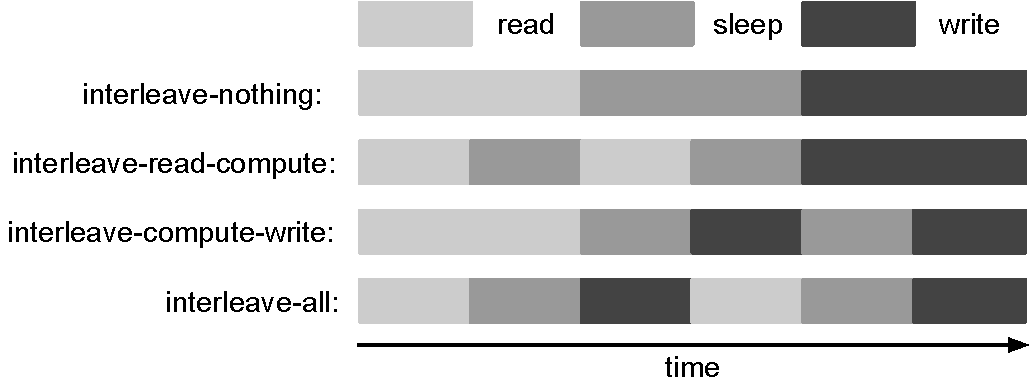
\includegraphics[width=85mm]{picture/Interleave}
\caption {Visualization of the Interleaving Options
    \label{fig:interleave}
}
\end{center}
\end{figure}

Line 17 in Listing~\ref{lst:bag} is a usage example of specifying the \textbf{Interleave\_Option}.

\subsection{Task Parameters}

The Skeleton tool's task is implemented by a versatile synthetic C program, where users can specify parameters to define
the computation and I/O behavior, if needed. (Note: this is optional; describing parameters for all tasks in a stage, as discussed in \S\ref{sec:stage-wide} 
will be sufficient for many application skeletons.)

The Skeleton task support two types: serial task and parallel task. 
A typical task specification looks like:
\begin{itemize}
\item[] Path\_to\_Task Task\_Type Num\_Processes Task\_Length Read\_Buffer Write\_Buffer Num\_Input Num\_Output Interleave\_Option [Input\_File] [Output\_File Output\_Size]
\end{itemize}
which could be filled in as:
\begin{itemize}
\item [] task serial 1 16 65536 65536 1 1 0 input\_file\ output\_file 1048576
\end{itemize}

\noindent The parameters of a task can be specified as:
\begin{itemize}
\item{\bf Task\_Type}: A user needs to declare \textbf{Task\_Type} to be either ``serial'' or ``parallel''
\item{\bf Num\_Processes}: If a task is declared to be ``serial'', \textbf{Num\_Processes} has to be specified as ``1''. If a task is declared to be ``parallel'', then \textbf{Num\_Processes} can be any integer value that is greater or equal to 1.
\item{\bf Task\_Length}: \textbf{Task\_Length} is specified in ``seconds''; it can be a integer or floating point number
\item{\bf Read\_Buffer}: \textbf{Read\_Buffer} specifies how much data the task reads as a chunk from storage. This parameter might be affected by file system buffer or other system settings
\item{\bf Write\_Buffer}: \textbf{Write\_Buffer} specifies how much data the task writes as a chunk to storage.This parameter might be affected by file system buffer or other system settings
\item{\bf Num\_Input}: Number of input files
\item{\bf Num\_Output}: Number of output files
\item{\bf Interleave\_Option}: Interleaving of input, output, and computation.
\item{\bf [Input\_File]}: A user needs to list all the input files in the task description. The number of input file names has to be compliant with the parameter \textbf{Num\_Input}
\item{\bf [Output\_File, Output\_Size]}: A user needs to list all output files with the file size strictly after each file name.
\end{itemize}


\section{Examples in GitHub}
This section explains the examples in the GitHub repository and their usage. The source code is available from \url{https://github.com/applicationskeleton/Skeleton/tree/master/src/sample-input}.
To run these examples, go to the ``src'' directory, then execute ``./skeleton.py sample-input/xxx.input Shell''.
\begin{itemize}
\item{\bf bag.input}: Generates a bag of independent tasks. 
\item{\bf two-stage.input}: Generates a two-stage application with file dependencies between the stages.
\item{\bf combination.input}: Generates a two-stage application with file dependencies as a combinatorial functions.
\item{\bf single-stage-iterative.input}: Generates an iterative application over one stage.
\item{\bf multiple-stage-iterative.input}: Generates an iterative application over multiple stages.
\item{\bf map-reduce.input}: Generates an map-reduce application.
\item{\bf sample.input}: Generates a multi-stage workflow application.
\item{\bf external-mapper.input}: Generates an two-stage application using the external mapper to specify task file mapping.
\item{\bf mapping.sh}: A example external script that prints the file mapping to standard output.
\end{itemize}

\section{Future work}

\begin{itemize}

\item{Site Specification}: Enables automatic or semi-automatic remote compiling and task deployment on multiple remote sites. 

\item{Error Reporting}: Enables error reporting in the application description file.

\item{Task dependencies}: Enables a task dependency purely on task sequence, not just through files.

\item{Concurrent tasks}: Enables multiple concurrent tasks that exchange files or data while running.


\end{itemize}

\section{Acknowledgments}

This work was funded by DOE ASCR under award DE-SC0008617.

\bibliographystyle{abbrv}
\bibliography{Skeleton}

\end{document}
